\part{Practical and Theoretical Foundations of Programming}
\label{intro}\toc

%%%%%%%%%%%%%%%%%%%%%%%%%%%%%%%%%%%%%%%%%%%%%%%%%%%%%%%%%%%%%%%%%%%%%%%%%% 
\section{Introduction}
\subsection{From the problem to the code}
\begin{frame}[t]{Problems}
  \null\vspace{-.7\baselineskip}
  \centerline{\includegraphics[subfig=1,scale=.8]{fig/algo_problem_program.fig}}

  \medskip
  \concept{Provided by clients (or teachers ;)}

  \begin{block}{Problems}
    \begin{itemize}
    \item \structure{Problems are generic}
    \item[] Example: Determine the minimal value of a set of integers
    \end{itemize}
  \end{block}

  \begin{block}{Instances of a problem}
    \begin{itemize}
    \item \structure{The problem for a given data set}
    \item[] Example: Determine the minimal value of \{17, 6, 42, 24\}
    \end{itemize}    
  \end{block}
\end{frame}
%%%%%%%%%%%%%%%%%%%%%%%%%%%%%%%%%%%%%%%%%%%%%%%%%%%%%%%%%%%%%%%%%%%%%%%%%% 
\begin{frame}[t,squeeze]{Problems and Programs}
  \centerline{\includegraphics[subfig=2,scale=.8]{algo_problem_program.fig}}

  \begin{block}{Software systems {\color{black} (\textit{ie.}, Programs)}}
    \begin{itemize}
    \item Describes a set of actions to be achieved in a given order
    \item Doable (tractable) by computers
    \end{itemize}
  \end{block}\vspace{-.5\baselineskip}

  \begin{block}<2->{Problem Specification}
    \begin{itemize}
    \item Must be clear, precise, complete, without ambiguities
    \item[] Bad example: find position of minimal element
      {\small (two answers for \{4, 2, 5, 2, 42\})}
    \item[] Good example: Let $L$ be the set of positions for which the value is minimal.\\
      ~~~~~~~~~~~~~~~~~~~~Find the minimum of $L$
    \end{itemize}
  \end{block}\vspace{-.5\baselineskip}

  \begin{block}<2->{Using the Right Models}
    \begin{itemize}
    \item Need simple models to understand complex artifacts (ex: city
      map)
    \end{itemize}
  \end{block}
\end{frame}
%%%%%%%%%%%%%%%%%%%%%%%%%%%%%%%%%%%%%%%%%%%%%%%%%%%%%%%%%%%%%%%%%%%%%%%%%% 
\begin{frame}[t,squeeze]{Methodological Principles}
  \centerline{\includegraphics[subfig=3,scale=.8]{algo_problem_program.fig}}

  \begin{block}{Abstraction
      \color{black}{\normalsize think before coding (!)}}
    \begin{itemize}
    \item Describe how to solve the problem
    \end{itemize}
  \end{block}\vspace{-.8\baselineskip}

  \begin{block}{Divide, Conquer and Glue 
      \color{black}{\normalsize(top-down approach)}}
    \begin{itemize}
    \item \structure{Divide} complex problem into simpler sub-problems
      (think of Descartes)
    \item \structure{Conquer} each of them
    \item \structure{Glue} (combine) partial solutions into the big one
    \end{itemize}
  \end{block}\vspace{-.8\baselineskip}

  \begin{block}{Modularity}
    \begin{itemize}
    \item Large systems built of components: \textbf{modules}
    \item Interface between modules allow to mix and match them
    \end{itemize}
  \end{block}
\end{frame}
%%%%%%%%%%%%%%%%%%%%%%%%%%%%%%%%%%%%%%%%%%%%%%%%%%%%%%%%%%%%%%%%%%%%%%%%%% 
\begin{frame}[t]{Algorithms}
  \centerline{\includegraphics[subfig=4,scale=.8]{algo_problem_program.fig}}
  
  \begin{block}{Precise description {\color{black}of the}
      resolution process {\color{black}of a} well specified problem}
    \begin{itemize}
    \item Must be understandable (by human beings)
    \item Does not depend on target programming language, compiler or machine
    \item Can be an diagram (as pictured), but difficult for large problems
    \item Can be written in a simple language (called \textbf{pseudo-code})
    \end{itemize}
  \end{block}
  
  \begin{block}{``Formal'' definition}
    \begin{itemize}
    \item Sequence of actions acting on problem data to induce the expected result
    \end{itemize}
  \end{block}
\end{frame}
%%%%%%%%%%%%%%%%%%%%%%%%%%%%%%%%%%%%%%%%%%%%%%%%%%%%%%%%%%%%%%%%%%%%%%%%%% 
\newcommand{\fleche}[1]{$\underrightarrow{\text{\hbox to 5cm{\hfill#1\hfill}}}$}
\begin{frame}[t]{New to Algorithms?}
  \begin{block}{Not quite, you use them since a long time}\bigskip
    \begin{tabular}{p{31mm} c l}
      Lego bricks\texttrademark&\fleche{list of pictures}&Castle\\\\
      Ikea\texttrademark\ desk&\fleche{building instructions}&Desk\\\\
      Home location&\fleche{driving directions}&Party location\\\\
      Eggs, Wheal, Milk&\fleche{recipe}&Cake\\\\
      Two 6-digits integers&\fleche{arithmetic know-how}&sum 
    \end{tabular}
  \end{block}

  \begin{block}{And now}\bigskip
    \begin{tabular}{p{31mm} c l}
      List of students&\fleche{sorting algorithm}&Sorted list\\\\
      Maze map&\fleche{appropriated algorithm}&Way out\\\\

    \end{tabular}    
  \end{block}
\end{frame}
%%%%%%%%%%%%%%%%%%%%%%%%%%%%%%%%%%%%%%%%%%%%%%%%%%%%%%%%%%%%%%%%%%%%%%%%%% 
\subsection{Computer Science vs. Software Engineering}
\begin{frame}{Computer Science vs. Software Engineering}
  \begin{boitequote}{}
    \alert{Computer science} is a science of abstraction – creating the right
    model for a problem and devising the appropriate mechanizable
    technique to solve it.\hfill -- {\rm Aho and Ullman}
  \end{boitequote}\bigskip

  \begin{block}{NOT (only) Science of Computers}\medskip
    \begin{boitequote}{}
      Computer science is not more related to computers than\\
      Astronomy to telescopes.\hfill--~{\rm Dijkstra}
    \end{boitequote}
      
    \begin{itemize}
    \item Many concepts were framed and studied before the electronic computer
    \item To the logicians of the 20's, a \textit{computer} was a person with
      pencil and paper
    \end{itemize}
  \end{block}

  \begin{block}{Science of Computing}
    \begin{itemize}
    \item Automated problem solving
    \item Automated systems that produce solutions
    \item Methods to develop solution strategies for these systems
    \item Application areas for automatic problem solving
    \end{itemize}
  \end{block}
\end{frame}
%%%%%%%%%%%%%%%%%%%%%%%%%%%%%%%%%%%%%%%%%%%%%%%%%%%%%%%%%%%%%%%%%%%%%%%%%% 
\begin{frame}{Foundations of Computing}
  \begin{block}{Fundamental mathematical and logical structures}
    \begin{itemize}
    \item To understand computing
    \item To analyze and verify the correctness of software and hardware
    \end{itemize}
  \end{block}

  \begin{block}{Main issues of interest in Computer Science}
    \begin{itemize}
    \item \structure{Calculability}
      \begin{itemize}
      \item Given a problem, can we show whether there exist an
        algorithm solving it?
      \item Which are the problems for which no algorithm exist? How to
        categorize them?
      \end{itemize}
    \item \structure{Complexity}
      \begin{itemize}
      \item How long does my algorithm need to answer? (as function
        of input size)
      \item How much memory does it take?
      \item Is my algorithm optimal, or does a better one exist?
      \end{itemize}
    \item \structure{Correctness}
      \begin{itemize}
      \item Can we be certain that a given algorithm always reaches a solution?
      \item Can we be certain that a given algorithm always reaches
        the right solution?
      \end{itemize}
    \end{itemize}
  \end{block}
\end{frame}
%%%%%%%%%%%%%%%%%%%%%%%%%%%%%%%%%%%%%%%%%%%%%%%%%%%%%%%%%%%%%%%%%%%%%%%%%% 
\begin{frame}{Software Engineering vs. Computer Science}
  \concept{Producing technical answers to consumers' needs}

  \begin{block}{Software Engineering Definition}
    \begin{itemize}
    \item Study of methods for producing and evaluating software
    \end{itemize}
  \end{block}
  
  \begin{block}<2->{Life cycle of a software
      {\color{black}\normalsize (\textit{much} more details to come later)}}\medskip
    \centerline{\includegraphics{fig/algo_cycleV.fig}}
    \begin{itemize}
    \item \structure{Global design:} Identify application modules
    \item \structure{Detailed design:} Specify within modules
    \end{itemize}
  \end{block}
\end{frame}
%%%%%%%%%%%%%%%%%%%%%%%%%%%%%%%%%%%%%%%%%%%%%%%%%%%%%%%%%%%%%%%%%%%%%%%%%% 
\begin{frame}{As future IT engineers, you need both CS and SE}
  \begin{block}{Without Software Engineering}
    \begin{itemize}
    \item Your production will not match consumers' expectation
    \item You will induce more bugs and problems than solutions
    \item Each program will be a pain to develop and to maintain for you
    \item You won't be able to work in teams
    \end{itemize}
  \end{block}

  \begin{block}{Without Computer Science}
    \begin{itemize}
    \item Your programs will run slowly, deal only with limited data sizes
    \item You won't be able to tackle difficult (and thus well paid) issues
    \item You won't be able to evaluate the difficulty of a task (and
      thus its price)
    \item You will reinvent the wheel (badly)
    \end{itemize}
  \end{block}

  \begin{block}<2->{Two approaches of the same issues}
    \begin{itemize}
    \item \structure{Correctness:}
      CS $\leadsto$ prove algorithms right; 
      SE $\leadsto$ chase (visible) bugs
    \item \structure{Efficiency:} CS $\leadsto$ theoretical bounds on
      performance, optimality proof;\\
      \hspace{16.6mm}SE $\leadsto$ optimize execution time and
      memory usage

    \end{itemize}
  \end{block}
\end{frame}
%%%%%%%%%%%%%%%%%%%%%%%%%%%%%%%%%%%%%%%%%%%%%%%%%%%%%%%%%%%%%%%%%%%%%%%%%% 
\section{Designing Algorithms for Complex Problems}\sectionpage
\begin{frame}{There are always several ways to solve a problem}
  \begin{block}<+->{Choice criteria between algorithms}
    \begin{itemize}
    \item \structure{Correctness:} provides the right answer
    \item \structure{\alert<+>{Simplicity:}}
      KISS! (jargon acronym for \textit{keep it simple, silly})
    \item \structure{Efficiency:} fast, use little memory
    \item \structure{Stability:} small change in input does not change output
    \end{itemize}
  \end{block}\vspace{-.5\baselineskip}

  \begin{block}<.->{Real problems ain't easy}
    \begin{itemize}
    \item They are not fixed, but \alert{dynamic}
      \begin{itemize}
      \item Specification helps users understanding the problem better\\
        That is why they often add wanted functionalities after specification
      \item My text editor is v23.2.1 
        {\small(hundreds of versions for ``just a text editor'')}
      \end{itemize}

    \item They are \alert{complex} (composed of several interacting entities)
    \end{itemize}
  \end{block}

  \visible<.->{
    \begin{boitequote}{\small"Epigrams in Programming", by Alan J. Perlis.}
      In computing, turning the obvious into the useful is a living definition
      of the word "frustration".
    \end{boitequote}
  }
\end{frame}
%%%%%%%%%%%%%%%%%%%%%%%%%%%%%%%%%%%%%%%%%%%%%%%%%%%%%%%%%%%%%%%%%%%%%%%%%% 
\begin{frame}{Dealing with Complexity}
  \begin{block}{Some classical design principles help}
    \begin{itemize}\vspace{-.2\baselineskip}
    \item \structure{Composition}: split problem in simpler
      sub-problems and compose pieces
    \item \structure{Abstraction}: forget about details and focus on
      important aspects
    \end{itemize}    
  \end{block}\vspace{-.5\baselineskip}

  \begin{block}{Object Oriented Programming}
    \begin{itemize}\vspace{-.2\baselineskip}
    \item Classical answer to specification complexity and dynamicity
      Encapsulation, polymorphism, heritage, \ldots
    % \item \structure{Encapsulation:} Divide complexity into manageable units
    % \item \structure{Polymorphism:} Use one (specialized) block instead of the
    %   expected one
    % \item \structure{Heritage:} Allow to factorize behavior between related
    %   units
    \item That's one way to \structure{design applications} in a modular manner
    \item Other approaches exists, but none have the same momentum currently
    \end{itemize}
  \end{block}\vspace{-.5\baselineskip}

  \visible<2>{
    \begin{block}{Rest of this module}
      \begin{itemize}%\vspace{-.2\baselineskip}
      \item How to write each block / units / objects to be composed in OOP
      \end{itemize}
    \end{block}\vspace{-.7\baselineskip}
    
    \begin{block}{Why algorithms before OOP and not the contrary?}
      \begin{itemize}\vspace{-.2\baselineskip}
      \item We just switched, to see how it works, now that Scala is usable
      \item Coding at small before programming at large
%      \item Every mainstream languages (including Java) are object oriented
%      \item Research in CS education shows that ``object first'' is a better
%        approach
      \end{itemize}
    \end{block}
  }
\end{frame}

%%%%%%%%%%%%%%%%%%%%%%%%%%%%%%%%%%%%%%%%%%%%%%%%%%%%%%%%%%%%%%%%%%%%%%%%%% 
\subsection{Composition}
\begin{frame}{Dealing with complexity: Composition}
  \begin{block}{Composite structure}
    \begin{itemize}
    \item \structure{Definition:} a software system composed of
      manageable pieces
    \item[\Smiley] The smaller the component, the easier it is to
      build and understand
    \item[\Frownie] The more parts, the more possible interactions
      there are between parts
    \item[$\Rightarrow$] the more complex the resulting structure
    \item Need to balance between simplicity and interaction minimization
    \end{itemize}
  \end{block}

  \begin{block}<2->{Good example: audio system}\medskip
    Easy to manage because:
    \begin{itemize}
    \item each component has a carefully specified function
    \item components are easily integrated
    \item i.e. the speakers are easily connected to the amplifier
    \end{itemize}
  \end{block}
\end{frame}

%%%%%%%%%%%%%%%%%%%%%%%%%%%%%%%%%%%%%%%%%%%%%%%%%%%%%%%%%%%%%%%%%%%%%%%%%% 
\begin{frame}[squeeze]{Composition counter-example (1/2)}
  \begin{block}{Rube Goldberg machines}
    \begin{itemize}
    \item Device not obvious, modification unthinkable
    \item Parts lack intrinsic relationship to the solved problem
    \item Utterly high complexity
    \end{itemize}
  \end{block} \vspace{-\baselineskip}

  \begin{columns}
    \begin{column}{.6\linewidth}
      \begin{block}{Example: Tax collection machine}\bigskip
        \includegraphics[width=\linewidth]{fig/algo_rube-localtaxes.fig}
      \end{block}
    \end{column}
    \begin{column}{.4\linewidth}
      \begin{enumerate}
      \item[A.] Taxpayer sits on cushion
      \item[B.] Forcing air through tube
      \item[C.] Blowing balloon
      \item[D.] Into candle
      \item[E.] Explosion scares dog
      \item[F.] Which pull leash
      \item[G.] Dropping ball
      \item[H.] On teeter totter
      \item[I.] Launch plans
      \item[J.] Which tilts lever
      \item[K.] Then Pitcher
      \item[L.] Pours water on plant
      \item[M.] Which grows, pulling chain
      \item[N.] Hand lifts the wallet
      \end{enumerate}    
    \end{column}
  \end{columns}
\end{frame}
%%%%%%%%%%%%%%%%%%%%%%%%%%%%%%%%%%%%%%%%%%%%%%%%%%%%%%%%%%%%%%%%%%%%%%%%%% 
\begin{frame}[squeeze]{Composition counter-example (2/2)}
  \begin{block}{Rube Goldberg's toothpaste dispenser}\smallskip
    \centerline{\includegraphics[width=.7\linewidth]{fig/algo_rube-toothpaste.fig}}
  \end{block}

  Such over engineered solutions should obviously remain jokes
\end{frame}
%%%%%%%%%%%%%%%%%%%%%%%%%%%%%%%%%%%%%%%%%%%%%%%%%%%%%%%%%%%%%%%%%%%%%%%%%% 
\subsection{Abstraction}
\begin{frame}{Dealing with complexity: Abstraction}
  \begin{block}{Abstraction}
    \begin{itemize}
    \item Dealing with components and interactions without worrying
      about details
    \item Not ``vague'' or ``imprecise'', but focused on few relevant properties
    \item Elimination of the irrelevant and amplification of the
      essential
    \item Capturing commonality between different things
    \end{itemize}
  \end{block}

  \begin{columns}
    \begin{column}{.3\linewidth}
      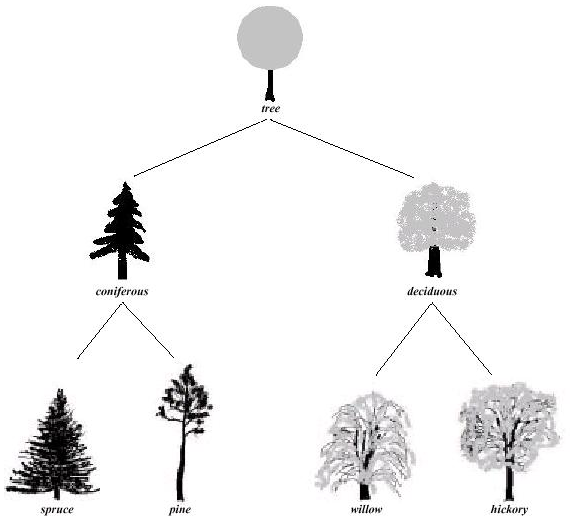
\includegraphics[width=\linewidth]{fig/algo_abstracting_trees.png}      
    \end{column}

    \begin{column}{.7\linewidth}
      \begin{block}<2->{Abstraction in programming}
        \begin{itemize}
        \item Think about what your components should do before
        \item Ie, abstract their \textbf{interface} before coding
        \visible<2->{
        \centerline{\includegraphics[scale=.8]{fig/algo_contract.fig}}~~~~~~~~~}
        \item Show your interface, hide your implementation
        \end{itemize}
      \end{block}
    \end{column}
  \end{columns}
  
\end{frame}
%%%%%%%%%%%%%%%%%%%%%%%%%%%%%%%%%%%%%%%%%%%%%%%%%%%%%%%%%%%%%%%%%%%%%%%%%% 
\section{Crash Course on Scala}\sectionpage
\begin{frame}{Scala? Why??}

  \begin{block}{Main reason for me: simplicity}
    \begin{itemize}
    \item Most of you are absolute beginners to programming
    \item I want to talk about algorithms, not to bother you about syntax
    \end{itemize}
  \end{block}

  \begin{block}{Scala has much more to offer}
    \begin{itemize}
    \item OOP (mixin+singleton), functional, properties, type inference, JVM-based \ldots
    \item<2-> But we don't care for now: \alert{see it as a simple language}
    \item<2-> You'll learn its true beauty later on
    \end{itemize}
  \end{block}
\end{frame}
%%%%%%%%%%%%%%%%%%%%%%%%%%%%%%%%%%%%%%%%%%%%%%%%%%%%%%%%%%%%%%%%%%%%%%%%%
\begin{frame}[fragile]{Starting Scala}
  
  \structure{\large Installation:} Get it from \url{http://scala-lang.org/} (version 2.10 at least)
  \smallskip

  \begin{block}{Executing your code}
    \begin{columns}
      \begin{column}{.28\linewidth}
        \begin{boitecode}{myfile.scala}
println("Hello, friends")

        \end{boitecode}
      \end{column}
      \begin{column}{.22\linewidth}
        \begin{boiteshell}{Run directly}
\$ scala myfile.scala          
Hello, friends
\$
        \end{boiteshell}
      \end{column}
      \begin{column}{.38\linewidth}
        \begin{boiteshell}{Compile first}
\$ scalac -Xscript toto myfile.scala          
\$ scala toto
Hello, friends
\$      \end{boiteshell}
      \end{column}
    \end{columns}
    %%%
    \begin{columns}
      \begin{column}{.3\linewidth}
        \begin{boitecode}{myscript}
#!/usr/bin/scala
!#
println("Hello, friends")
        \end{boitecode}
        \begin{boiteshell}{Turn it into a script}
\$ chmod +x myscript
\$ ./myscript
Hello, friends
\$      \end{boiteshell}
      \end{column}
      \begin{column}{.4\linewidth}
        \begin{boiteshell}{Run interactively}
\$ scala
Welcome to Scala [...]

scala> \structure{println("Hello, friends")}
Hello, friends

scala> \structure{:load myfile.scala}
Loading toto.scala...
Hello, friends
        \end{boiteshell}
      \end{column}

    \end{columns}
  \end{block}
\end{frame}
%%%%%%%%%%%%%%%%%%%%%%%%%%%%%%%%%%%%%%%%%%%%%%%%%%%%%%%%%%%%%%%%%%%%%%%%%%%%
\begin{frame}{Getting Started in Scala}
  \structure{\large Declaring a variable:} {\large\framebox{\texttt{var x:Int = 0}} }
  \smallskip

  \begin{tabular}{c@{~$\leadsto$~}l}
    \texttt{var} & because that's a \textbf{var}iable\\
    \texttt{x}   & name of that variable (its label)\\
    \texttt{:Int}& type of this variable (what it can store)\\
    \texttt{= 0}  & initial value (mandatory)
  \end{tabular}

  \begin{itemize}
  \item You can often omit the type (it's inferred): \framebox{\texttt{var x = 0}}
  \end{itemize}

  \begin{block}{Some Scala data types}
    \begin{itemize}
    \item \structure{Int:} for integer values,  \structure{Double:} for dot numbers
    \item \structure{Boolean:} \texttt{true/false}, \structure{String:} \texttt{"some chars together"}
    \end{itemize}
  \end{block}

  \begin{block}<2->{Declaring a value}
    \begin{itemize}
    \item If your "variable" is constant, make it a value:
      ~\framebox{\texttt{\alert{val} answer:Int = 42}}
      \smallskip
      
    \item Seen as good style in Scala \hfill%
      \textit{\small mutable stateful objects are the new spaghetti code}
    \item Allows to detect errors, may produce faster code, easy multithreading.
    \item Do values unless you must use variables
    \end{itemize}
  \end{block}

\end{frame}
%%%%%%%%%%%%%%%%%%%%%%%%%%%%%%%%%%%%%%%%%%%%%%%%%%%%%%%%%%%%%%%%%%%%%%%%%%%%
\begin{frame}[fragile]{The Scala Syntax}
  \begin{block}{Looping}\smallskip
  \begin{columns}
    \begin{column}{.3\linewidth}
      \begin{Verbatim}[gobble=8,fontsize=\small,frame=single,commandchars=+[\]]
        +textrm[+textbf[while]] (+textit[condition]) {
          +textit[instructions]
        }
      \end{Verbatim}
    \end{column}

    \begin{column}{.3\linewidth}
      \begin{Verbatim}[gobble=8,fontsize=\small,frame=single,commandchars=+[\]]
        +textrm[+textbf[do]] {
          +textit[instructions]
        } +textrm[+textbf[while]] (+textit[condition])
      \end{Verbatim}
    \end{column}

    \begin{column}{.37\linewidth}
      \begin{Verbatim}[gobble=8,fontsize=\small,frame=single,commandchars=+[\]]
        +textrm[+textbf[for]] (+textit[i] +textrm[+textbf[+recvVal]] 0 +textrm[+textbf[to]] 10 +textrm[+textbf[by] 2]) {
          // i in 0,2,4,6,8,10
        }
      \end{Verbatim}
    \end{column}
  \end{columns}
  \end{block}

  \bigskip
  \begin{block}{Methods and functions}\smallskip
    \begin{columns}
      \begin{column}{.37\linewidth}
        \begin{Verbatim}[gobble=9,fontsize=\small,frame=single,commandchars=+[\]]
         +textrm[+textbf[def]] +textit[sayIt](msg:String) {
           print(msg)
         }
        \end{Verbatim}
      \end{column}

      \begin{column}{.55\linewidth}
        \begin{Verbatim}[gobble=9,fontsize=\small,frame=single,commandchars=+[\]]
         +textrm[+textbf[def]] +textit[max3](x:Int, y:Int, z:Int)+alert[:Int =] {
           val m = if (x>y) x else y
           if (m>z) {
             return m
           } else {
             return z
           }
         }
        \end{Verbatim}
      \end{column}
    \end{columns}
  \end{block}
\end{frame}
%%%%%%%%%%%%%%%%%%%%%%%%%%%%%%%%%%%%%%%%%%%%%%%%%%%%%%%%%%%%%%%%%%%%%%%%%%%%%%
\begin{frame}[fragile]{Pattern matching: cascading if / else if are over}
  
  \begin{columns}
    \begin{column}{.57\linewidth}
      \begin{Verbatim}[gobble=8,fontsize=\footnotesize,frame=single,commandchars=+[\]]
        +textit[name] +textrm[+textbf[match]] {
          +textrm[+textbf[case]] +textit["Martin"] => +textit[println("Hey there")]
          +textrm[+textbf[case]] +textit["Gerald"] => +textit[println("Hello")]
          +textrm[+textbf[case]] _ +hspace[10.7mm]=> +textit[println("Gnii?")]
        }
      \end{Verbatim}
    \end{column}
    \begin{column}{.42\linewidth}
      \begin{itemize}
      \item Veeery powerful construct
      \item Any expression can be filtered
      \item The default case is mandatory
      \end{itemize}
    \end{column}
  \end{columns}

  \begin{columns}
    \begin{column}{.73\linewidth}
      \begin{Verbatim}[gobble=8,fontsize=\footnotesize,frame=single,commandchars=+[\]]
        +textit[name] +textrm[+textbf[match]] {
          +textrm[+textbf[case]] +textit["Martin"] | +textit["Gerald"] => +textit[println("Hey there")]
          +textrm[+textbf[case]] _ +hspace[27.7mm]=> +textit[println("Gniii?")]
        }
      \end{Verbatim}      
    \end{column}
    \begin{column}{.265\linewidth}
      ~
    \end{column}
  \end{columns}

 \begin{columns}
    \begin{column}{.73\linewidth}
      \begin{Verbatim}[gobble=8,fontsize=\footnotesize,frame=single,commandchars=+[\]]
        +textit[age] +textrm[+textbf[match]] {
          +textrm[+textbf[case]] i +textrm[+textbf[if]] i<20 => println("Hey dude!")
          +textrm[+textbf[case]] i +textrm[+textbf[if]] i<30 => println("Hello young man")
          +textrm[+textbf[case]] _ +hspace[11.4mm]=> println("Hello Sir")
        }
      \end{Verbatim}      
    \end{column}
    \begin{column}{.265\linewidth}
      ~
    \end{column}
  \end{columns}

 \begin{columns}
    \begin{column}{.73\linewidth}
      \begin{Verbatim}[gobble=8,fontsize=\footnotesize,frame=single,commandchars=+[\]]
        +textit[(x,y)] +textrm[+textbf[match]] {
          +textrm[+textbf[case]] (0,0) => println("Origin")
          +textrm[+textbf[case]] (_,0) => println("Abscissa")
          +textrm[+textbf[case]] (0,_) => println("Ordinate")
          +textrm[+textbf[case]] (_,_) => println("Random")
        }
      \end{Verbatim}      
    \end{column}
    \begin{column}{.265\linewidth}
      ~
    \end{column}
  \end{columns}
\end{frame}
%%%%%%%%%%%%%%%%%%%%%%%%%%%%%ù
\begin{frame}

  \Concept{There is much more to Scala}
  \medskip

  \centerline{But that's all you need to know for now\ldots}
\end{frame}

\section{Comparing Algorithms' Efficiency}\sectionpage
\begin{frame}{Comparing Algorithms' Efficiency}
  \concept{There are always more than one way to solve a problem}
  \begin{block}<+->{Choice criteria between algorithms}
    \begin{itemize}
    \item \structure{Correctness:} provides the right answer
    \item \structure{Simplicity:} \textit{not} Rube Goldberg's machines 
    \item \alert{Efficiency:} fast, use little memory
    \item \structure{Stability:} small change in input does not change output
    \end{itemize}
  \end{block}\vspace{-.5\baselineskip}

  \begin{block}<+->{Empirical efficiency measurements}
    \begin{itemize}
    \item Code the algorithm, benchmark it and use runtime statistics
    \item[\Frownie] Several factors impact performance: \\
      {\small machine, language, programmer, compiler, compiler's options,
      operating system, \ldots}
    \item[$\Rightarrow$] Performance not generic enough for comparison
    \end{itemize}
  \end{block}\vspace{-.5\baselineskip}

  \begin{block}<+->{Mathematical efficiency estimation}
    \begin{itemize}
    \item Count amount of basic instruction as function of input size
    \item[\Smiley] Simpler, more generic and often sufficient
    \item[] {\small(true in theory;
      in practice, optimization necessary \textbf{in addition} to this)}
    \end{itemize}
  \end{block}
\end{frame}
%%%%%%%%%%%%%%%%%%%%%%%%%%%%%%%%%%%%%%%%%%%%%%%%%%%%%%%%%%%%%%%%%%%%%%%%%% 
\subsection{Best case, worst case, average analysis}
\begin{frame}[fragile,squeeze]{Best case, worst case, average analysis}
  \concept{Algorithm running time depends on the data}
  \begin{block}<+->{Example: Linear search in an array}\vspace{-.5\baselineskip}
    \begin{center}      
    \begin{minipage}{.7\linewidth}
    \begin{Verbatim}[frame=single,fontsize=\footnotesize,gobble=6]
      def linearSearch(val:Int, tab:Array[Int]): Boolean = {
        for (i <- 0 to tab.length-1) 
          if (tab(i) == val)
            return true;
        return false
      }
    \end{Verbatim}      
    \end{minipage}
    \end{center}\vspace{-.8\baselineskip}
    \begin{itemize}
    \item Case 1: search whether 42 is in \{42, 3, 2, 6, 7, 8, 12, 16, 17, 32, 55, 44, 12\}\\
      answer found after one step
    \item Case 2: search whether 4 is in \{42, 3, 2, 6, 7, 8, 12, 16, 17, 32, 55, 44, 12\}\\
      need to traverse the whole array to decide (n steps)
    \end{itemize}
  \end{block}\vspace{-.5\baselineskip}

  \begin{block}<+->{Counting the instructions to run in each case}
    \begin{itemize}
    \item $t_{min}$: \#instructions for the best case inputs 
    \item $t_{max}$: \#instructions for the worst case inputs 
    \item $t_{avg}$: \#instructions  on average 
      {\small(average of values coefficiented by probability)}\\
      $t_{avg}=p_1t_1+p_2t_2+\ldots+p_nt_n$
    \end{itemize}
  \end{block}
\end{frame}
%%%%%%%%%%%%%%%%%%%%%%%%%%%%%%%%%%%%%%%%%%%%%%%%%%%%%%%%%%%%%%%%%%%%%%%%%% 
\begin{frame}[fragile]{Linear search runtime analysis}
  \begin{center}\vspace{-.6\baselineskip}      
    \begin{minipage}{.6\linewidth}
    \begin{Verbatim}[frame=single,fontsize=\footnotesize,gobble=6]
        for (i <- 0 to tab.length-1)
          if (tab(i) == val)
            return true
        return false
    \end{Verbatim}      
    \end{minipage}
    \end{center}\vspace{-.3\baselineskip}

    \begin{itemize}
    \item For simplicity, let's assume the value is in the array,
      positions are equally likely
    \item Let's count tests (noted \alert{t}), 
      additions (noted \alert{a}) and 
      value changes (noted \alert{c})
    \end{itemize}


  \begin{block}{Best case: searched data in first position}
    \begin{itemize}
    \item 1 value change (i=0); 2 tests  (loop boundary + equality)
    \item $ t_{min}=\alert{c}+2\alert{t}$
    \end{itemize}
  \end{block}\vspace{-.5\baselineskip}
  \begin{block}{Worst case: searched data in last position}
    \begin{itemize}
    \item 1 value change (i=0); \{2 tests, 1 change, 1 addition (i+=1)\} per loop
    \item $t_{max}=c+n\times(2t+1c+1a)=(n+1)\times\alert{c}+2n\times\alert{t}+n\times\alert{a}$
    \end{itemize}
  \end{block}\vspace{-.5\baselineskip}

  \begin{block}<2->{Average case: searched data in position $p$ with
      probability $\frac{1}{n}$}
    \begin{itemize}
    \item {\small$\displaystyle t_{avg}
        =c+\sum_{p\in[1,n]}\frac{1}{n}\times (2t+c+a)\times p
        \uncover<3->{=c+\frac{1}{n}\times(2t+c+a)\times\sum_{p\in[1,n]}p}$}\\
      {\small$\uncover<4->{\displaystyle t_{avg}
        =c+\frac{n(n-1)}{2n}\times(2t+c+a)}
        \uncover<5->{
        =(n-1)\times\alert{t}+\frac{n+1}{2}\times\alert{c}+\frac{n-1}{2}\times\alert{a}}
        $}
    \end{itemize}
  \end{block}
\end{frame}
%%%%%%%%%%%%%%%%%%%%%%%%%%%%%%%%%%%%%%%%%%%%%%%%%%%%%%%%%%%%%%%%%%%%%%%%%% 
\begin{frame}{Simplifying equations}
  \concept{\fbox{$t_{avg}=(n-1)\times t+\frac{n+1}{2}\times
      c+\frac{n-1}{2}\times a$} is too complicated}

  \begin{block}<2->{Reducing amount of variables}
    \begin{itemize}
    \item To simplify, we only count the most expensive operations
    \item But which it is is not always clear...
    \item Let's take write accesses \alert{c} (classical but arbitrary choice)
    \end{itemize}
  \end{block}

  \begin{block}<3->{Focusing on dominant elements}
    \begin{itemize}
    \item We can forget about constant parts if there is n operations
    \item We can forget about linear parts if there is $n^2$ operations
    \item \ldots
    \item Only consider the most dominant elements when
      $n$ is very big
    \item[$\Rightarrow$] This is called \textbf{\alert{asymptotic complexity}}
    \end{itemize}
  \end{block}
\end{frame}
%%%%%%%%%%%%%%%%%%%%%%%%%%%%%%%%%%%%%%%%%%%%%%%%%%%%%%%%%%%%%%%%%%%%%%%%%% 
\subsection{Asymptotic complexity}
\begin{frame}{Asymptotic Complexity: Big-O notation}
  \begin{block}{Mathematical definition}
    \begin{itemize}
    \item Let $T(n)$ be a non-negative function
    \item \fbox{$T(n) \in O(f(n))$} 
      $\Leftrightarrow \exists \text{ constants } c, n_0 
      \text{ so that } \forall n>n_0,$ \fbox{$T(n)\le c\times f(n)$}
    \item f(n) is an upper bound of T(n) \ldots
    \item[\ldots] after some point, and with a constant multiplier
    \end{itemize}
  \end{block}

  \begin{block}{Application to runtime evaluation}
    \begin{itemize}
    \item $T(n)\in O(n^2)\Rightarrow$ when n is big enough, you need less than $n^2$ steps
    \item This gives a upper bound
    \end{itemize}
  \end{block}
\end{frame}
%%%%%%%%%%%%%%%%%%%%%%%%%%%%%%%%%%%%%%%%%%%%%%%%%%%%%%%%%%%%%%%%%%%%%%%%%% 
\begin{frame}[fragile]{Big-O examples}
  \begin{block}{Example 1: Simplifying a formula}
    \begin{itemize}
    \item Linear search: $t_{avg}=(n-1)\times t+\frac{n+1}{2}\times
      c+\frac{n-1}{2}\times a$ $\Rightarrow$ \framebox{$T(n)=O(n)$}
    \item Imaginary example: $T(n)=17n^2+\frac{32}{17}n+\pi$
      $\Rightarrow$ \framebox{$T(n)=O(n^2)$}
    \item If T(n) is constant, we write T(n)=O(1)
    \end{itemize}
  \end{block}

  \begin{block}{Practical usage}
    \begin{itemize}
    \item Since this is a upper bound, $T(n)=O(n^3)$ is also true when $T(n)=O(n^2)$
    \item But not as relevant
    \end{itemize}
  \end{block}

  \begin{block}<2->{Example 2: Computing big-O values directly}\medskip
    \begin{center}
      \begin{minipage}{.5\linewidth}        
      \begin{Verbatim}[label=array initialization,gobble=8,frame=single]
        for (i <- 0 to tab.length-1) 
          tab(i) = 0
      \end{Verbatim}
      \end{minipage}
    \end{center}
    \vspace{-\baselineskip}
    \begin{itemize}
    \item We have $n$ steps, each of them doing a constant amount of work
    \item $T(n) = c\times n$ ~~ $\Rightarrow$ ~~ $T(n) = O(n)$
    \item[] (don't bother counting the constant elements)
    \end{itemize}
  \end{block}
\end{frame}
%%%%%%%%%%%%%%%%%%%%%%%%%%%%%%%%%%%%%%%%%%%%%%%%%%%%%%%%%%%%%%%%%%%%%%%%%% 
\begin{frame}{Big-Omega notation}
  \begin{block}{Mathematical definition}
    \begin{itemize}
    \item Let $T(n)$ be a non-negative function
    \item \fbox{$T(n) \in \Omega(f(n))$} 
      $\Leftrightarrow \exists \text{ constants } c, n_0 
      \text{ so that } \forall n>n_0,$ \fbox{$T(n)\ge c\times f(n)$}
    \item Similar to Big-O, but gives a \alert{lower} bound
    \item Note: similarly to before, we are interested in big lower bounds
    \end{itemize}
  \end{block}

  \begin{block}{Example: $T(n)=c_1\times n^2+c_2\times n$}
    \begin{itemize}
    \item $T(n)=c_1\times n^2+c_2\times n\ge c_1\times n^2$ ~~~ $\forall n>1$\\
      $T(n)\ge c\times n^2$ for $c>c_1$
    \item Thus, $T(n)=\Omega(n^2)$
    \end{itemize}
  \end{block}
\end{frame}
%%%%%%%%%%%%%%%%%%%%%%%%%%%%%%%%%%%%%%%%%%%%%%%%%%%%%%%%%%%%%%%%%%%%%%%%%% 
\begin{frame}{Theta notation}
  \begin{block}{Mathematical definition}
    \begin{itemize}
    \item $T(n)\in\Theta(g(n))$ if and only if 
      $T(n)\in O(g(n))$ and $T(n)\in\Omega(g(n))$
    \end{itemize}
  \end{block}

  \centerline{\includegraphics[scale=1.3]{fig/algo_theta.fig}}

  \begin{block}{Example}\vspace{-\baselineskip}
    \begin{center}      
      \resizebox{.7\linewidth}{!}{\begin{tabular}{l|c|c|c|c|c}\cline{2-5}
      \multicolumn{1}{l}{}&
      \multicolumn{1}{|l|}{}&
      n=10&n=1000&n=100000\\\cline{2-5}

      \multirow{2}*{$\Theta(n)$}&n&10&1000&$10^5$&\multirow{2}*{seconds}\\
      &100n&1000&$10^5$&$10^7$\\
      \cline{2-5}

      \multirow{2}*{$\Theta(n^2)$}&$n^2$&100&$10^6$&$10^{10}$
      &\multirow{2}*{minutes}\\
      &$100n^2$&$10^4$&$10^8$&$10^{12}$\\
      \cline{2-5}

      \multirow{2}*{$\Theta(n^3)$}&$n^3$&1000&$10^9$&$10^{15}$
      &\multirow{2}*{hours}\\
      &$100n^2$&$10^5$&$10^{11}$&$10^{17}$\\
      \cline{2-5}

      \multirow{2}*{$\Theta(2^n)$}&$2^n$&1024&$>10^{301}$&$\infty$
      &\multirow{2}*{\ldots}\\
      &$100\times 2^n$&$>10^5$&$10^{305}$&$\infty$\\
      \cline{2-5}

      \multirow{2}*{$\log(n)$}&$\log(n)$&3.3&$9.9$&$16.6$&\\
      &$100\log(n)$&$332.2$&$996.5$&$1661$\\
      \cline{2-5}
    \end{tabular}}
    \end{center}
  \end{block}
\end{frame}
%%%%%%%%%%%%%%%%%%%%%%%%%%%%%%%%%%%%%%%%%%%%%%%%%%%%%%%%%%%%%%%%%%%%%%%%%% 
\begin{frame}{Classical mistakes}
  \begin{block}<+->{Mistake notations}
    \begin{itemize}
    \item Indeed, we have  $O(\log(n))=O(n)=O(n^2)=O(n^3)=O(2^n)$ \\
      \visible<+->{{\small Because it's an upper bound; to be correct we should
          write $\subset$ instead of =}}
    \item Likewise, we have
      $\Omega(\log(n))=\Omega(n)=\Omega(n^2)=\Omega(n^3)=\Omega(2^n)$\\
      \visible<.->{{\small Because it's a lower bound; we should write
          $\supset$ instead of =}}
    \item We only have  $\Theta(\log(n))\neq\Theta(n)\neq\Theta(n^2)
      \neq\Theta(n^3)\neq\Theta(2^n)$\vspace{.3\baselineskip}
    \visible<+->{
    \item[] (but in practice, everybody use O() as if it were $\Theta()$ --
      although that's wrong)}
    \end{itemize}
  \end{block}

  \begin{block}<+->{Mistake worst case and upper bounds}
    \begin{itemize}
    \item Worst case is the input data leading to the longest operation time
    \item Upper bound gives indications on increase rate when input size
      increases 
    \item[] (same distinction between best case and lower bound)
    \end{itemize}
  \end{block}
\end{frame}
%%%%%%%%%%%%%%%%%%%%%%%%%%%%%%%%%%%%%%%%%%%%%%%%%%%%%%%%%%%%%%%%%%%%%%%%%% 
\begin{frame}{Asymptotic Complexity in Practice}
  \begin{block}{Rules to compute the complexity of an algorithm}
    \begin{description}
    \item[Rule 1:] Complexity of a sequence of instruction: Sum of
      complexity of each
    \item[Rule 2:] Complexity of basic instructions (test, read/write
      memory): O(1)
    \item[Rule 3:] Complexity of \texttt{if}/\texttt{switch}
      branching: Max of complexities of branches
    \item[Rule 4:] Complexity of loops: Complexity of content $\times$
      amount of loop
    \item[Rule 5:] Complexity of methods: Complexity of content
    \end{description}
  \end{block}\vspace{-.5\baselineskip}

  \begin{block}<2->{Simplification rules}\vspace{-.3\baselineskip}
    \begin{itemize}
    \item \structure{Ignoring the constant}:
    \item[] If f(n) = O({\small $k\times g(n)$}) 
            and $k>0$ is constant
            then f(n) = O(\small{g(n)})
    \item \structure{Transitivity}
    \item[] If f(n) = O({\small g(n)}) 
            and g(n) = O({\small h(n)}) 
            then f(n) = O(\small{h(n)})
    \item \structure{Adding big-Os}
    \item[] If A(n) = O({\small f(n)}) 
            and B(n) = O({\small g(n)}) 
            then A(n)+B(n) = O(\small{max({\footnotesize f(n), g(n)})})\\
            \hspace{77.7mm}= O({\small f(n)+g(n)})\vspace{-.7\baselineskip}
    \item \structure{Multiplying big-Os}
    \item[] If A(n) = O({\small f(n)}) 
            and B(n) = O({\small h(n)}) 
            then $A(n)\times B(n)$ = O({\small $f(n)\times g(n)$})
    \end{itemize}
  \end{block}
\end{frame}
%%%%%%%%%%%%%%%%%%%%%%%%%%%%%%%%%%%%%%%%%%%%%%%%%%%%%%%%%%%%%%%%%%%%%%%%%% 
\begin{frame}[fragile]{Some examples}
  \begin{block}{Example 1: {\color{black}\normalsize
      \fbox{\texttt{a=b;}} $\Rightarrow \Theta(1)$ (constant time)}}
  \end{block}\vspace{-\baselineskip}

  \begin{block}{Example 2}\vspace{-\baselineskip}
    \begin{columns}
      \begin{column}{.1\linewidth}~\end{column}
      \begin{column}{.3\linewidth}
        \begin{Verbatim}[gobble=8]
        var sum=0;
        for (i <- 1 to n)
          sum += n;
      \end{Verbatim}
      \end{column}
      \begin{column}{.3\linewidth}
        $\Theta(n)$
      \end{column}
    \end{columns}
  \end{block}

  \begin{block}{Example 3}\vspace{-\baselineskip}
    \begin{columns}
      \begin{column}{.1\linewidth}~\end{column}
      \begin{column}{.3\linewidth}
        \begin{Verbatim}[gobble=8]
        var sum=0;
        for (i <- 1 to n)
          for (j <- 1 to n)
            sum += 1
        for (k <- 0 to n-1)
          A(k) = k;
      \end{Verbatim}
      \end{column}
      \begin{column}{.3\linewidth}
        $\Theta(1)+\Theta(n^2)+\Theta(n)=\Theta(n^2)$
      \end{column}
    \end{columns}
  \end{block}

  \begin{block}{Example 4}\vspace{-\baselineskip}
    \begin{columns}
      \begin{column}{.1\linewidth}~\end{column}
      \begin{column}{.3\linewidth}
        \begin{Verbatim}[gobble=8]
        var sum=0;
        for (i <- 1 to n)
          for (j <- 1 to i)
            sum += 1
      \end{Verbatim}
      \end{column}
      \begin{column}{.3\linewidth}
        $\Theta(1)+O(n^2)=O(n^2)$
        one can also show $\Theta(n^2)$
      \end{column}
    \end{columns}
  \end{block}

  \begin{block}{Example 5}\vspace{-\baselineskip}
    \begin{columns}
      \begin{column}{.1\linewidth}~\end{column}
      \begin{column}{.3\linewidth}
        \begin{Verbatim}[gobble=8]
        var sum=0; var i=0
        while (i<n) {
          sum +=1
          i = i * 2
        }
      \end{Verbatim}
      \end{column}
      \begin{column}{.3\linewidth}
        $\Theta(\log(n))$
        $\log$ is due to the $i\times2$
      \end{column}
    \end{columns}
  \end{block}
\end{frame}
%%%%%%%%%%%%%%%%%%%%%%%%%%%%%%%%%%%%%%%%%%%%%%%%%%%%%%%%%%%%%%%%%%%%%%%%%% 
\begin{frame}{Going further on Algorithm Complexity}
  \vspace{-.5\baselineskip}
  \begin{block}<+->{Problems' Classification}
    \begin{itemize}\vspace{-.2\baselineskip}
    \item Problems can also be sorted in class of complexities (not only
      algorithms)\\
      {\small depending on the best existing algorithm to solve them}
    \item Showing that no better algorithm exist for a given problem:
      \alert{Calculability}
    \item Multi-million question: \alert{P=NP?}
      \begin{description}
      \item[P:] polynomial algorithm to find the solution exists
      \item[NP:] {\small candidate solution eval. in polynomial time, but no
          known polynomial algo}
      \item[NP-complete:] set of NP problems for which if one P algorithm is
        found, \\
        it's applicable to every other NP-complete problems
      \end{description}
    \end{itemize}
  \end{block}\vspace{-.5\baselineskip}

  \begin{block}<+->{\alert{Time} is not the only metric of interest:
      \alert{Space} too}
    \begin{itemize}\vspace{-.2\baselineskip}
    \item In computation, there is a sort of tradeoff between space and time\\
      {\small  Faster algorithms need to pre-compute elements \ldots
        requiring more storage memory}
    \end{itemize}
  \end{block}\vspace{-.5\baselineskip}

  \begin{block}<+->{So does \alert{Energy} nowadays!}
    \begin{itemize}\vspace{-.2\baselineskip}
    \item Computational power of CPU grows linearly with frequency;\\
      Energy consumption grows (more than) quadratically with frequency
    \item To save energy (and money), split your task on several
      slower cores \\
      {\small Parallel algorithms are the way to go (but it's \textit{ways}
        harder)}
    \end{itemize}
  \end{block}
\end{frame}
%%%%%%%%%%%%%%%%%%%%%%%%%%%%%%%%%%%%%%%%%%%%%%%%%%%%%%%%%%%%%%%%%%%%%%%%%% 
\section{Algorithmic Stability}\sectionpage
\begin{frame}[fragile]{Algorithmic stability}

  \begin{block}{Computers use fixed precision numbers}
    \begin{itemize}
    \item<+-> 10+1=11
    \item<+-> $10^{10}+1=10000000001$
    \item<+-> $10^{16}+1=10000000000000001$
    \item<+-> $10^{17}+1=10000000000000000\alert{0}=10^{17}$
    \end{itemize}
  \end{block}

  \begin{block}<+->{What is the value of $\sqrt{2^2}$?}
    \begin{itemize}
    \item Old computers though it was 1.9999999
    \end{itemize}
  \end{block}

  \begin{block}<.->{Other example}
    \begin{columns}
      \begin{column}{.27\linewidth}
        \begin{Verbatim}[gobble=9]
          while (value < 2E9) 
            value += 1E-8;
        \end{Verbatim}
      \end{column}
      \begin{column}{.6\linewidth}
        This is an infinite loop\\
        {\small(because when $value=10^9$, $value+10^{-8}=value$)}
      \end{column}
    \end{columns}
  \end{block}

  \medskip
  \uncover<+->{
  \concept{Numerical instabilities are to be killed to predict weather,}

  \concept{simulate a car crash or control a nuclear power plant}}

  \medskip\uncover<+->{(but this is all \textit{ways} beyond our goal this year ;)}
\end{frame}
%%%%%%%%%%%%%%%%%%%%%%%%%%%%%%%%%%%%%%%%%%%%%%%%%%%%%%%%%%%%%%%%%%%%%%%%%% 
\section{Conclusion}
\begin{frame}[squeeze]{Conclusion of this chapter}
  ~\vspace{-1.5\baselineskip}
  \begin{block}<+->{What tech guys tend to do when submitted a problem}
    \vspace{-.4\baselineskip}
    \begin{itemize}
    \item They code it directly, and rewrite everything once they
      understood
    \item And rewrite everything to improve performance
    \item And rewrite everything when the code needs to evolve
    \end{itemize}
  \end{block}\vspace{-.6\baselineskip}

  \begin{block}<+->{What managers tend to do when submitted a problem}
    \vspace{-.4\baselineskip}
    \begin{itemize}
    \item They write up a long and verbose specification
    \item They struggle with the compiler in vain
    \item Then they pay a tech guy 
      {\small(and pay too much since they don't get the grasp)}
    \end{itemize}
  \end{block}\vspace{-.6\baselineskip}

  \begin{block}<+->{What theoreticians tend to do when submitted a problem}
    \vspace{-.4\baselineskip}
    \begin{itemize}
    \item They write a terse but formal specification
    \item They write an algorithm, and prove its optimality
    \item[] (the algorithm never gets coded)
    \end{itemize}
  \end{block}\vspace{-.6\baselineskip}

  \begin{block}<+->{What good programmers do when submitted a problem}
    \vspace{-.4\baselineskip}
    \begin{itemize}
    \item They write a clear specification
    \item They come up with a clean design
    \item They devise efficient data structures and algorithms
    \item Then (and only then), they write a clean and efficient code
    \item They ensure that the program does what it is supposed to do
    \end{itemize}
  \end{block}
\end{frame}
%%%%%%%%%%%%%%%%%%%%%%%%%%%%%%%%%%%%%%%%%%%%%%%%%%%%%%%%%%%%%%%%%%%%%%%%%% 
\begin{frame}[squeeze]{Choice criteria between algorithms}
  \begin{block}{Correctness}
    \begin{itemize}
    \item \structure{Provides the right answer}
    \item This crucial issue is delayed a bit further
    \end{itemize}
  \end{block}\vspace{-.6\baselineskip}
  \begin{block}{Simplicity}
    \begin{itemize}
    \item \structure{Keep it simple, silly}
    \item Simple programs can evolve (problems and client's wishes often do)
    \item Rube Goldberg's machines cannot evolve
    \end{itemize}
  \end{block}\vspace{-.6\baselineskip}
  \begin{block}{Efficiency}
    \begin{itemize}
    \item \structure{Run fast, use little memory, dissipate little energy}
    \item Asymptotic complexity must remain polynomial
    \item Note that you cannot have a decent complexity with the wrong
      data structure
    \item You still want to test the actual performance of your code in practice
    \end{itemize}
  \end{block}\vspace{-.6\baselineskip}
  \begin{block}{Numerical stability}
    \begin{itemize}
    \item \structure{Small change in input does not change output}
    \item Advanced issue, critical for numerical simulations (but beyond our
      scope)
    \end{itemize}
  \end{block}
\end{frame}